\documentclass{beamer}
\usepackage{amsfonts, amsmath, graphicx, verbatim, graphicx}
\usetheme{Warsaw}

\title{Imputation Methodology for FAOSTAT Production Domain}
\author{\it Michael. C. J.  Kao}
\institute{Food and Agriculture Organization \\of the United Nation}
\date{}


\AtBeginSection[]
{
  \begin{frame}<beamer>
    \frametitle{Outline for section \thesection}
    \tableofcontents[currentsection]
  \end{frame}
}

\begin{document}

\frame{
  \titlepage
}

\begin{frame}
  \frametitle{Outline}
  \tableofcontents
\end{frame}



\begin{frame}
  \frametitle{Why do we need imputation?}

  The agricultural production domain is integral to the compilation of
  Food Balance Sheets. In particular to estimate consistent food
  supplies, imputation is required to ensure that data are non-sparse.
  Owing to the potential impact of imputation when often data are
  missing, accuracy and reliability of food estimates cannot be
  compromised.
  
  \vspace{0.5cm}
  The relationship of production and its components can be expressed as:

  \begin{equation}
    P_t = A_t \times Y_t
  \end{equation}
  
  Where $P_t$, $A_t$ and $Y_t$ denotes production, area harvested and
  yield, respectively, at time $t$.

\end{frame}  


\section{Current Methodology}

\begin{frame}

  The presently applied methodology aims to capture the variation of relevant
  commodity and/or geographic characteristics through the application
  of aggregated growth rates. a five-hierachy was designated represented 
  by:

  \begin{enumerate}
    \item Same country/commodity aggregate
    \item Sub-region aggregate/same commodity
    \item Sub-region aggregate/commodity aggregate
    \item Regional aggregate/same commodity
    \item Regional aggregate/commodity aggregate
  \end{enumerate}

\end{frame}

\begin{frame}

  In short, the aggregation imputation method computes the
  commodity/regional aggregated growth of both area and production,
  the growth rate is then applied to the last observed value. The
  formulae of the aggregated growth can be expressed as:
  
  \begin{equation}
    \label{eq:aggregateGrowth}
    r_{s, t} = \sum_{c \in \mathbb{S}} X_{c, t}/\sum_{c \in \mathbb{S}} X_{c, t-1}
  \end{equation}
  
  The imputation can then be computed as:
  \begin{equation}
    \hat{X}_{c, t} = X_{c, t-1} \times r_{s, t}
  \end{equation}
  
\end{frame}

\begin{frame}
  There are several shortcomings of the current methodology,
  \begin{itemize}
  \item Divergence of area and production, there are mainly two reasons for this.
    \begin{enumerate}
      \item Due to missing values, the aggregated growth can be heavily biased.
      \item The basket used to compute the aggregated growth rate is
        not the same over time and between area and production.
    \end{enumerate}
  \item Assumes perfect correlation between group and country series.
  \item Cannot support and incorporate additional information.
  \end{itemize}
\end{frame}

%% \section{Case Study and Exploratory Data Analysis}

%% \frame{

%%   To illustrate the proposed imputation, we have chosen Wheat from the
%%   crop group and Cassava from the root group as case studies. Both are important
%%   agricultural products but Wheat is much more commercialised and traded
%%   than is Cassava.

%%   \vspace{0.5cm}
  
%%   We have log-transformed the data to make the relationsihp an
%%   additive one, so that the production can be decomposed.
  
%%   \begin{equation}
%%     \log(P_t) = \log(A_t) + \log(Y_t)
%%   \end{equation}

%% }


%% \frame{
%%   \frametitle{Area dictates the level and changes in the production}
%%   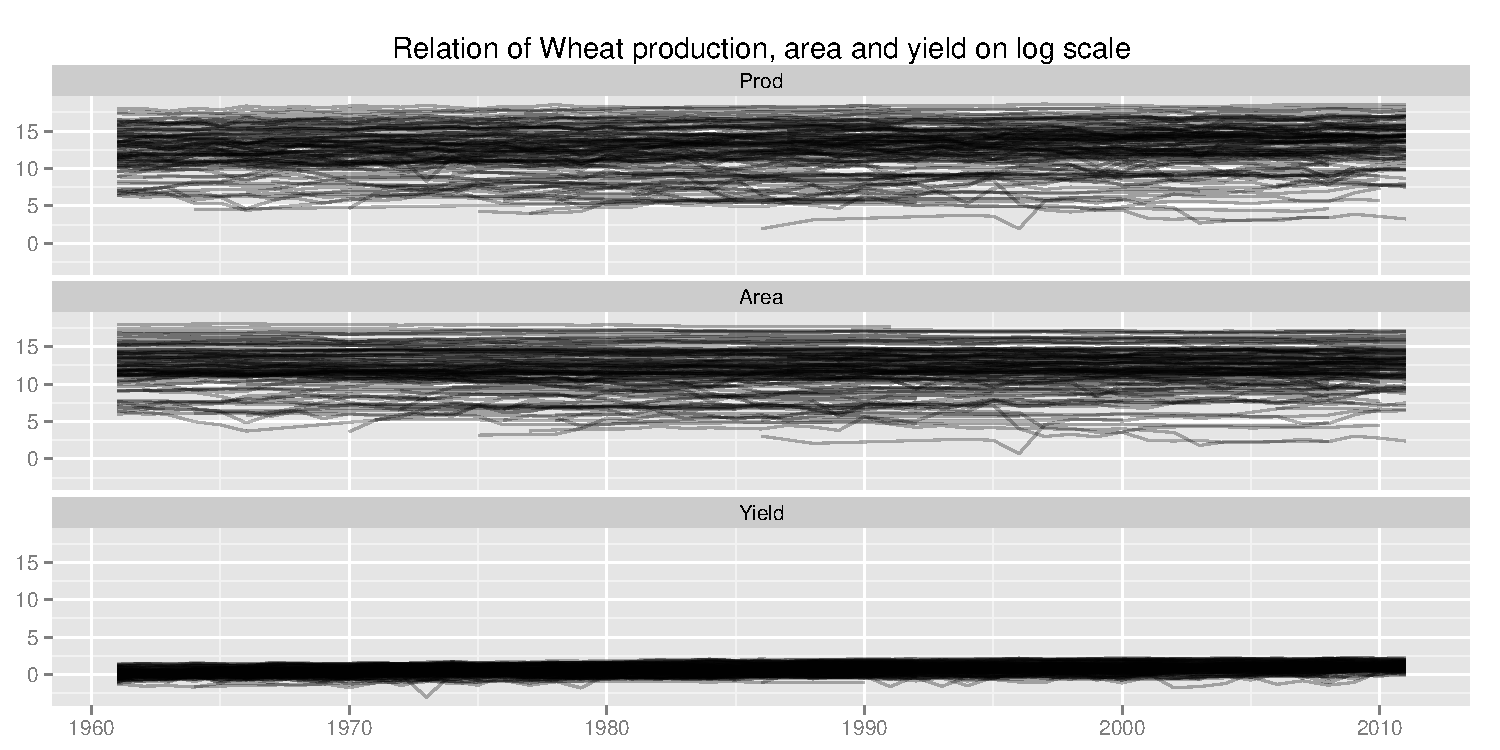
\includegraphics[scale = 0.45]{wheatIdentityBreakDown}
%% }

%% \frame{
%%   \frametitle{Same for Cassava}
%%   \includegraphics[scale = 0.45]{cassavaIdentityBreakDown}
%% }

%% \frame{
%%   \frametitle{Let us dig deeper}
%%   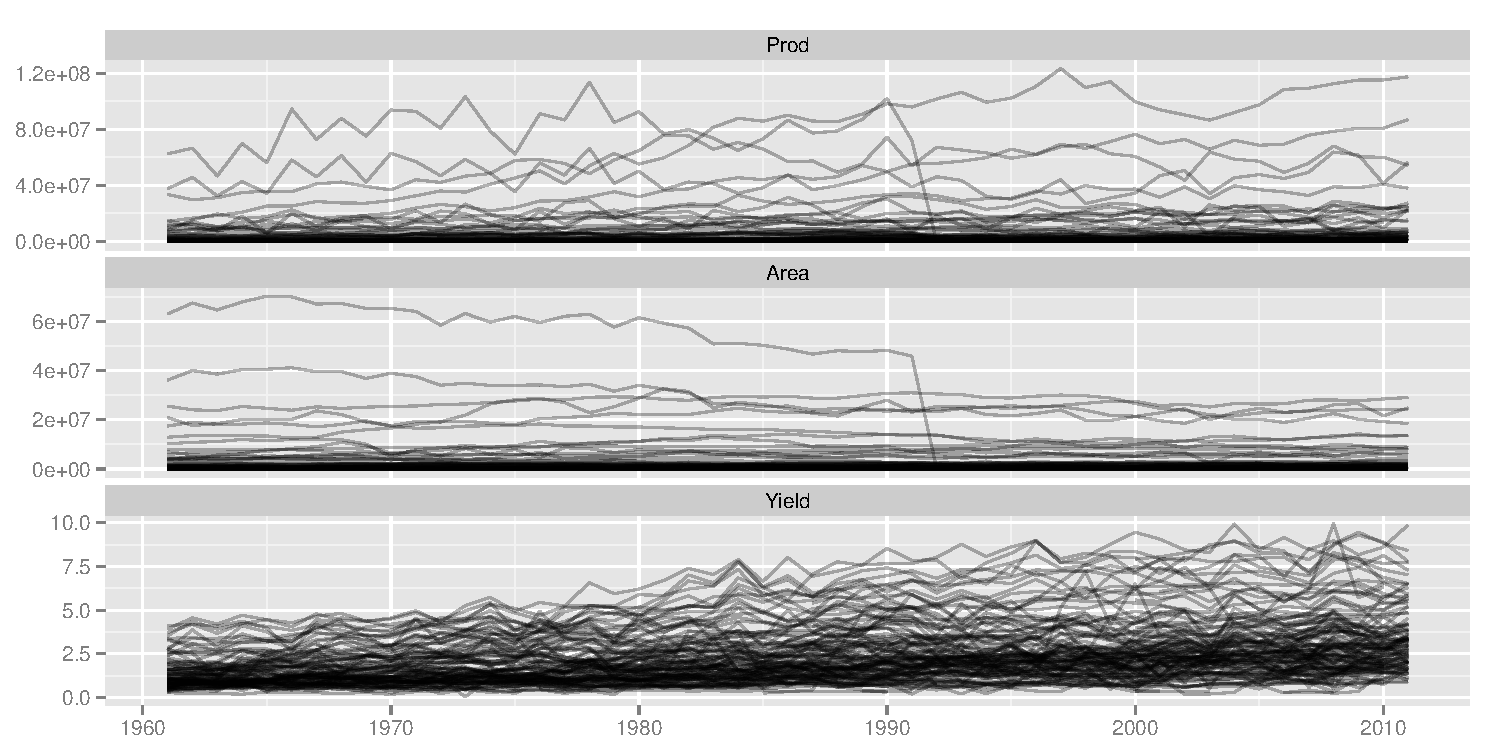
\includegraphics[scale = 0.45]{wheatAreaYield}
%% }

%% \frame{
%%   \frametitle{The co-movement appears weaker}
%%   \includegraphics[scale = 0.45]{cassavaAreaYield}
%% }

%% \frame{
%%   \frametitle{What is the data telling us?}

%%   What the data have shown is that the level, trend of the production
%%   is mainly determined by a smooth monotonic area occasionally
%%   affected by shocks, while the yield generates the variation from
%%   year-to-year reflecting climate or economic conditions.

%%   \vspace{0.5cm}
  
%%   This leads to the proposed methodology to estimate the year-to-year
%%   variation of yield while a stable method for area.

%% }


\section{Proposed Methodology}

\frame{

  In the new methodology, we propose to impute the yield and area, and along with
  the restriction of the new model this almost guarantees that area
  and production will not diverge.\\
  \vspace{0.5cm}
  Second, instead of applying the changes directly, the model
  estimates the relationship between the country and the aggregated
  series and applies the factors accordingly.\\
  \vspace{0.5cm}  
  Finally the proposed model allows incorporation of additional
  information such as prices, vegetation indices and other data that may
  improve the accuracy of the imputation.

}
\subsection{Imputation for Area Harvested}
\frame{

  Currently we have adopted \textbf{linear interpolation} and
  \textbf{last observation carry forward} to impute area
  harvestd. This is what we called the naive imputation.
  
  \vspace{0.5cm}

  First the area harvested and particularly carcass weight per animal
  displays close to monotonic behaviour and much little year-to-year
  fluctuation and thus linear interpolation is suitable. Furthermore,
  a previous simulation study has shown linear interpolation gives
  best result.

  %% \vspace{0.5cm} 

  %% While "last observation carry forward" is useful when the last
  %% observed value is a true zero, we will not impute a positive value.

  %% \vspace{0.5cm}

  %% We are, however, investigating improvements in the imputation of area
  %% harvested using information such as area sown.

}


\subsection{Imputation for Yield}
\frame{
  \frametitle{Linear Mixed Model}

  To capture the co-movement of yield and model sub-regional
  differences, we have proposed to model the yield with a Linear Mixed
  Model (LME), which can be expressed as follows in matrix notation:

  \begin{align}
    \mathbf{y_i} &= \mathbf{X_i}\boldsymbol{\beta} +
    \mathbf{Z_i}\mathbf{b_i} + \epsilon_i \nonumber\\
    \mathbf{b_i} &\sim \mathbf{N_q}(\mathbf{0}, \boldsymbol{\Psi})\nonumber\\
    \epsilon_i &\sim \mathbf{N_{ni}}(\mathbf{0},
    \boldsymbol{\sigma^2}\boldsymbol{\Lambda_i})
  \end{align}
  
}

\frame{
  
  More specifically, the equation for the imputation is
  \begin{align}
    \label{eq:lmeImpute}
  \text{Y}_{i,t} &= \overbrace{\beta_{0j} + \beta_{1j}t}^{\text{Fixed
      effect}} + \overbrace{b_{0,i} + b_{1,i}t +
    b_{2,i, t}\bar{Y}_{j,t}}^{\text{Random effect}} + \epsilon_{i,t}
  \end{align}

  The average yield can be calculated as follow,

  \begin{align}
    \label{eq:averageYield}
    \bar{Y}_{j, t} = \sum_{i \in j} \omega_i Y_{i,t}
  \end{align}

  Which acts as a proxy to reflect the change in climatics conditions
  and other factors which can simultaneously affect multiple
  countries. However, due to missing values, this quantity is not
  computed directly from the raw data. The EM-algorithm is implemented
  for the estimation for the unbiased average.

}

\frame{
  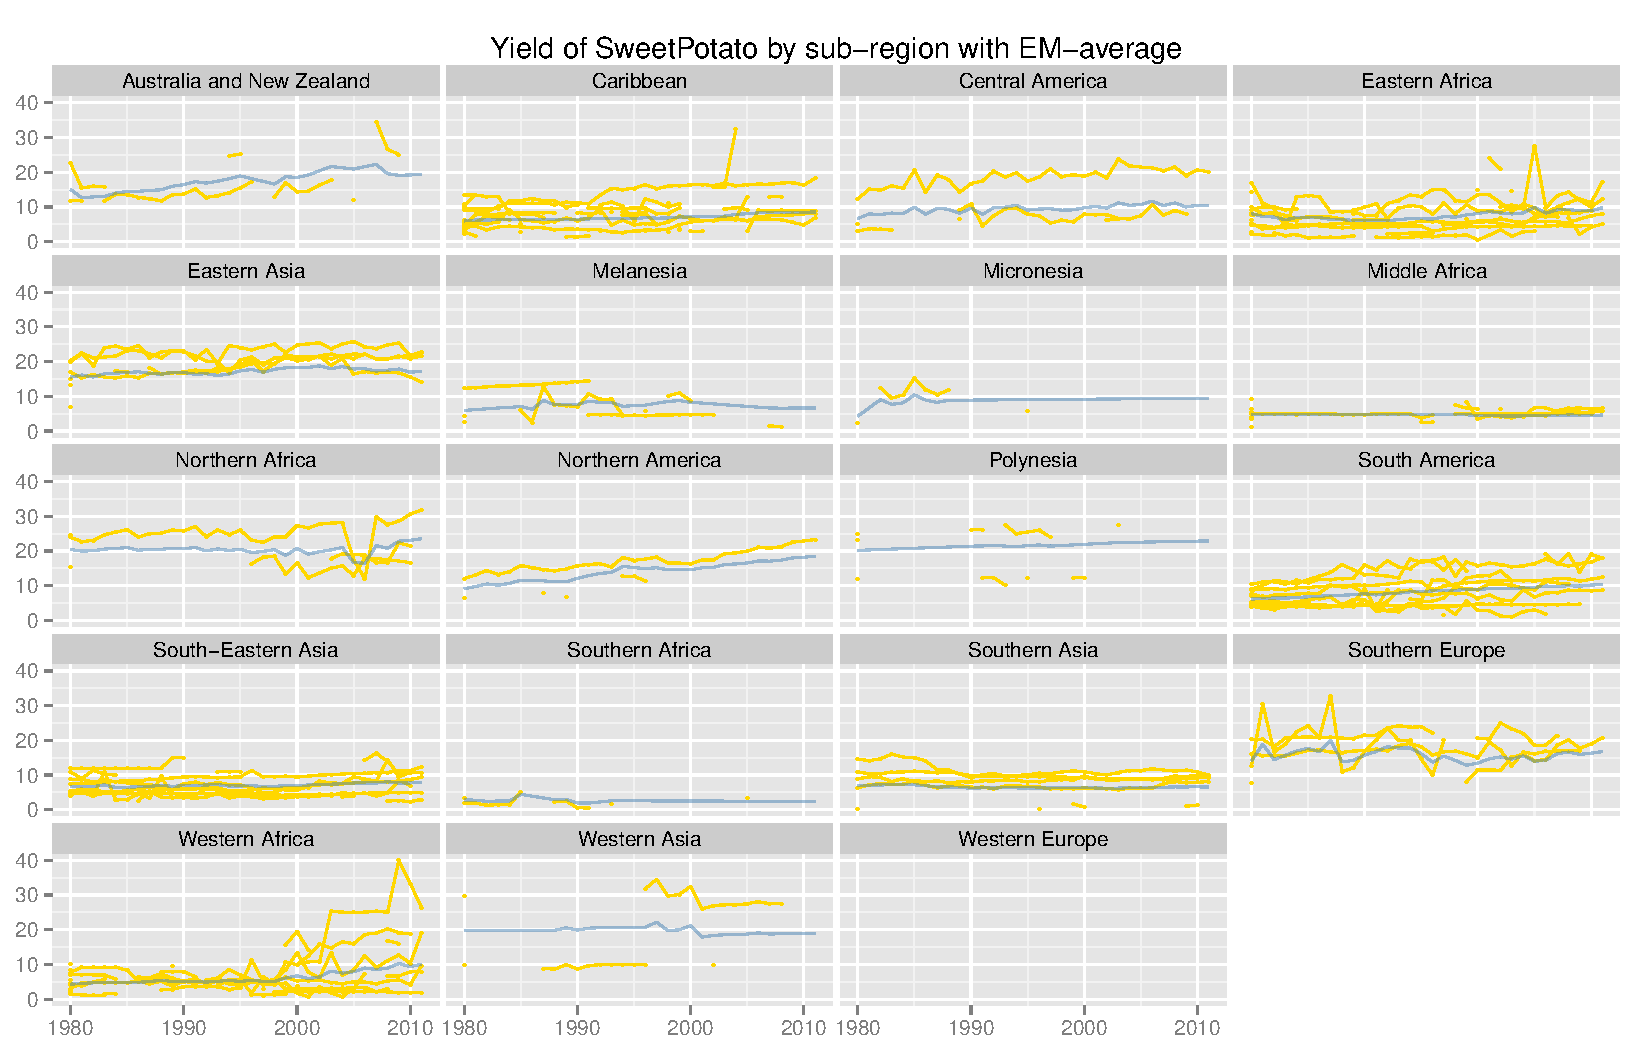
\includegraphics[scale = 0.4]{sweetPotatoYieldSubregion}
}


%% \frame{
%%   \includegraphics[scale = 0.4]{cassavaYieldSubregion}
%% }


\section{Results}

\subsection{Individual imputation}

\frame{
  \includegraphics[page = 18, scale = 0.4]{checkSweetPotatoImputation}
}


\frame{
  \includegraphics[page = 57, scale = 0.4]{checkSweetPotatoImputation}
}

\frame{
  \includegraphics[page = 90, scale = 0.4]{checkSweetPotatoImputation}
}

\frame{
  \includegraphics[page = 104, scale = 0.4]{checkSweetPotatoImputation}
}


\frame{
  \includegraphics[page = 108, scale = 0.4]{checkSweetPotatoImputation}
}

\subsection{Simulation Results}
\frame{
  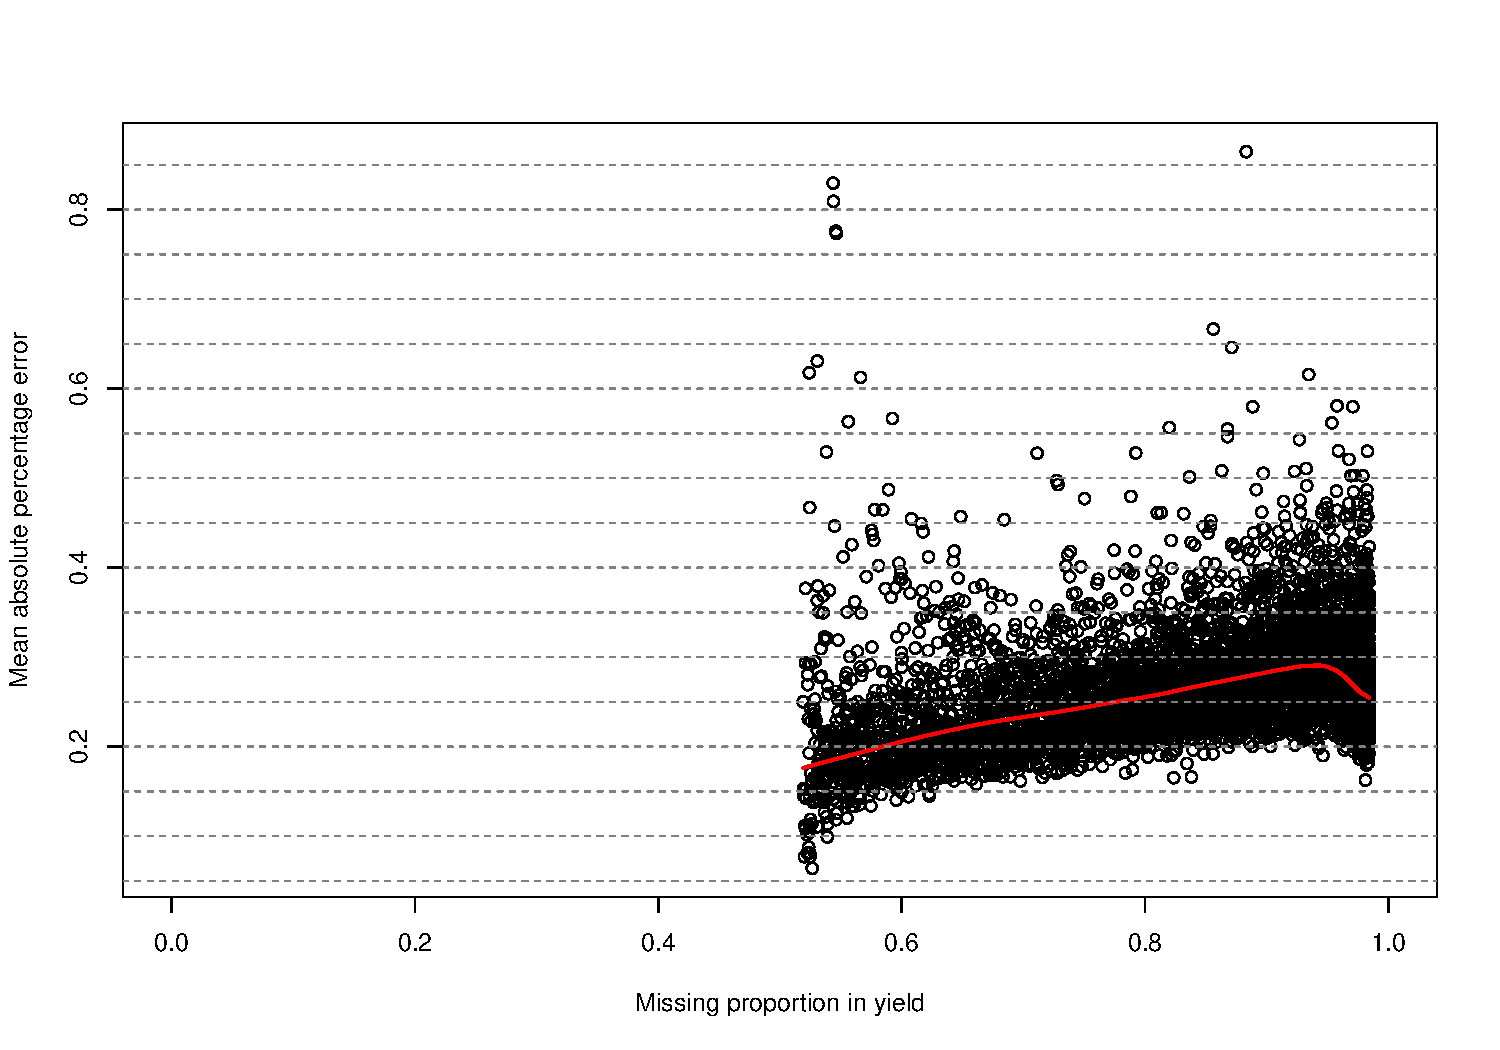
\includegraphics[scale = 0.4]{sweetPotatoSimulationResult}
}


%% \frame{
%%   \includegraphics[page = 20, scale = 0.4]{checkWheatImputation}
%% }



%% \subsection{Results for Cassava}
%% \frame{
%%   \includegraphics[page = 23, scale = 0.4]{checkCassavaImputation}
%% }

%% \frame{
%%   \includegraphics[page = 15, scale = 0.4]{checkCassavaImputation}
%% }

%% \frame{
%%   \includegraphics[page = 36, scale = 0.4]{checkCassavaImputation}
%% }

%% \frame{
%%   \includegraphics[page = 14, scale = 0.4]{checkCassavaImputation}
%% }


%% \frame{
%%   \includegraphics[page = 92, scale = 0.4]{checkCassavaImputation}
%% }


%% \section{Further Improvements}
\section{Discussion}
\frame{

\begin{itemize}
  \item Incorporation additional information for imputation.
  \item Develope a better grouping classification.
\end{itemize}

  Thank you for your time and attention.

}

%% \frame{
%% \includegraphics[scale = 0.3]{EMmeanCheck}
%% }


%% \frame{

%%   The newly proposed methodology demonstrates the ability to resolve
%%   issues in the current methodology and extended to incorporate
%%   additional information.

%%   \vspace{0.5cm}
%%   We welcome any information which can enhance the performance of the
%%   imputation.
%%   \vspace{0.5cm}

%% }


\end{document}
